\section{FPGA Design}

In this section, we explain our design decisions and details of the FPGA implementations. The device targeted is a Xilinx Artix-7 FPGA, although the design is not device specific and is generic enough to comfortably fit on most low-cost FPGA devices. The generic design also applies to the parameter sets, meaning the design ideals are the same for both \textsf{FrodoKEM-640} and \textsf{FrodoKEM-976}. We propose a design that aims to balance between FPGA area consumption and throughput / runtime of the operations. There are separate designs for key generation, encapsulation, and decapsulation, since we expect an embedded device to usually compute these operations separately.  

\subsection{Overview} \label{sec:frodo_fpga}

The FPGA designs of all three cryptographic operations consist of three main components: matrix-matrix multiplication, addition of an error distribution, and the use of random oracles via cSHAKE. Our designs use two cSHAKE modules and one AES module. Essentially all the designs proposed have the same critical path, that is, the matrix-matrix multiplications. All other modules, such as random number generation, occur in parallel to this which saves significant clock cycles and simplifies the overall design. This also means the clock cycles per operation are easily calculable and, more importantly, happen in \emph{constant time}, where for example, encapsulation happens in $\hat{n} \times ( n \times \hat{n} + \hat{n} \times \hat{n} )$ clock cycles. Efficient constant runtime is a practical countermeasure to some simple side-channel attacks such as timing analysis.

Instead of creating a hardware module for matrix-matrix multiplication, we instead utilize a vector-matrix multiplier which loops over the $\bar{n}=8$ rows of the $\mathbf{S}^\prime$ matrix, for calculating both $\mathbf{B}^\prime$ and $\mathbf{V}$ matrices (i.e., for encapsulation in Algorithm \ref{alg:encaps}). This equivalent operation saves area consumption by not requiring all of $\mathbf{S}^\prime$ to be stored, as once each row of $\mathbf{S}^\prime$ is used, that corresponding row of $\mathbf{S}^\prime$ is not needed again. This is true for both encapsulation and decapsulation, where $\mathbf{S}^\prime$ is required to be reused in more than one multiplication instance.

Many of the operations within \textsf{FrodoKEM} key generation, encapsulation, and decapsulation are similar, with some differences in the use of encoding or decoding. More specifically, the main key generation operations also lie in encapsulation, and decapsulation, and (with the exception of calculating $\mathbf{M}$) encapsulation and decapsulation also share many of the same operations. These similarities will also be seen by the similar results of area consumption on the FPGA, due to the use of the same sub-modules. Thus, the operations of encapsulation will be described, where a high-level overview of the architecture is given in Figure \ref{fig:fpga}.

\textsf{FrodoKEM} encapsulation begins with an initialization stage. This step is required mainly for reading in the public-key information onto the device. This time required is exploited to also initialize the cSHAKE module (used for generating $\mathbf{A}$), generating the uniformly random key $\mu$, and pre-generating some of the matrix $\mathbf{A}$. The public-key ($\mathbf{B}$) information and the matrix $\mathbf{A}$ are stored in block RAM (BRAM), and are called upon in the multiplication component depending on a row-column (address) count. 

Once the initialization has finished, the computation of the matrix $\mathbf{B}^\prime$ starts, requiring a vector of values from the error distribution, a matrix of uniform values, and another error distribution value used for addition. The differences in these error distribution values is that the first, used in $\mathbf{S}^\prime$, is required again for the multiplication of $\mathbf{V}$, and is hence stored, whereas those required for the addition of $\mathbf{E}^\prime$ and $\mathbf{E}^{\prime\prime}$ are not required again and are not stored for further use. Once a single row of $\mathbf{S}^\prime$ is generated, the next row is generated in parallel to the running of the multiplication of $\mathbf{B}^\prime$, where a double-buffered store (sometimes called the page-flip method or ping-pong buffering) is used. At the end of each vector-matrix operation ($\bar{n}=8$ of these are required), the buffers are then swapped. Using this technique saves 4x in the storage requirements of $\mathbf{S}^\prime$ and ensures there is no delay between any of the vector-matrix multiplication operations in the LWE multiplier.

An encapsulation operation is complete when the vector-matrix LWE multiplier has looped over the $\bar{n}=8$ vectors of $\mathbf{S}^\prime$, for calculating $\mathbf{B}^\prime$ and $\mathbf{V}$. As the coefficients of these matrices become available, they are input into a second cSHAKE module, used as a random oracle to calculate the shared secret $\mathbf{ss}$. This stage is computed in parallel to the next encapsulation operation, which simplifies the overall design and ensures the constant runtime.

%\begin{figure}
%\resizebox{\textwidth}{!}{%
%\noindent\makebox[\textwidth]{
%%\renewcommand{\arraystretch}{1.2}
%\footnotesize
%\centering
%\begin{tabular}{l|c|c|c|c|c|c|c|}
% %\setlength\extrarowheight{-3pt}
% \cline{2-4}
% KEM $\sharp 1$  & Mult.~$\mathbf{B}^\prime$ $\Rightarrow$ & Mult.~$\mathbf{V}$ $\Rightarrow$ & Comp.~$\mathbf{ss}$ &  \multicolumn{4}{c}%{} \\ \cline{2-6}
% \multicolumn{1}{l}{KEM $\sharp 2$} & \multicolumn{2}{c|}{} & Mult.~$\mathbf{B}^\prime$ $\Rightarrow$ & Mult.~$\mathbf{V}$ $\Rightarrow$ %& Comp.~$\mathbf{ss}$ & \multicolumn{2}{c}{} \\ \cline{4-6}
% \multicolumn{1}{c}{$\vdots$} & \multicolumn{1}{c}{} & \multicolumn{3} {r} {} & \multicolumn{1}{l}{$\ddots$} & \multicolumn{1}{r}{}  \\ %\cline{6-8}%
% \multicolumn{1}{l}{KEM $\sharp n$} & \multicolumn{4}{c|}{} & Mult.~$\mathbf{B}^\prime$ $\Rightarrow$ & Mult.~$\mathbf{V}$ $\Rightarrow$ & Comp.~$\mathbf{ss}$ \\ \cline{6-8}
%\end{tabular}}}
%\caption{A high-level overview of the pipeline incorporated within the Encapsulation (and Decapsulation) algorithm of \textsf{FrodoKEM}.}
%\label{fig:frodo_pipe}
%\end{figure}

\subsection{LWE Multiplication Core} \label{sec:lwe_core}

At the center of the \textsf{FrodoKEM} FPGA design is a LWE multiplication core which consists of vector-matrix multiplication and addition of the error distribution and, if required, the message data. The generic design generates and stores a single row of the error matrix $\mathbf{S}^\prime$ for use in the calculation of $\mathbf{B}^\prime$ and $\mathbf{V}$. Whilst these operations are taking place the next row of $\mathbf{S}^\prime$ is being generated, and the vectors are swapped at the end of each vector-matrix multiplication. This process loops for $\bar{n}=\bar{m}=8$ rows, the same for both parameter sets. 

The design exploits a DSP block on the FPGA device, as it matches the requirements of the vector-matrix multiplications; a 25-by-18 bit multiplier and a 48-bit accumulator. Each vector loop of $\mathbf{S}^\prime$ is multiplied by a matrix (either $\mathbf{A}$ or $\mathbf{B}$) and adds an error distribution value and, if required, message data of the encoding of $\mu$. The nature of the DSP means that each multiplication within the MAC happens in a single clock cycle, ensures constant runtime, and makes the clock cycles counts easily calculable since the MAC operations are the critical path of the proposed designs. Figure \ref{fig:frodo_pipe} shows the pipelines of each vector-matrix MAC operation, as well as the parallelising of these with the additions required.


\begin{figure}
\resizebox{\textwidth}{!}{%
\centering
\begin{tabular}{l|c|c|c|c|c|}
 %\setlength\extrarowheight{-3pt}
 \cline{2-4}
 MAC 1 & MAC$(\mathbf{S}^\prime[\text{row}],\mathbf{A}[\text{col}])$ & Add error $\mathbf{E}^\prime$ & Output & \multicolumn{2}{c}{} \\ \cline{2-5}
 \multicolumn{1}{l}{MAC 2} & \multicolumn{1}{c|}{} & MAC$(\mathbf{S}^\prime[\text{row}],\mathbf{A}[\text{col}])$ & Add error $\mathbf{E}^\prime$ & Output & \multicolumn{1}{c}{} \\ \cline{3-5}
 \multicolumn{1}{c}{$\vdots$} & \multicolumn{1}{c}{} & \multicolumn{1} {r} {} & \multicolumn{1}{c}{$\ddots$} & \multicolumn{2}{r}{}  \\ \cline{4-6}
 \multicolumn{1}{l}{MAC $n$} & \multicolumn{2}{c|}{} & MAC$(\mathbf{S}^\prime[\text{row}],\mathbf{A}[\text{col}])$ & Add error $\mathbf{E}^\prime$ & Output \\ \cline{4-6}
\end{tabular}}
\caption{A high-level overview of the pipeline incorporated within the LWE multiplication core, for example $\mathbf{B} = \mathbf{S}^\prime \mathbf{A} + \mathbf{E}^\prime$. Latency is minimised due to parallelising the multiply-accumulate (MAC) operations within the DSP and additions with the error.}
\label{fig:frodo_pipe}
\end{figure}


  \begin{figure}[H]
  	\centering
  	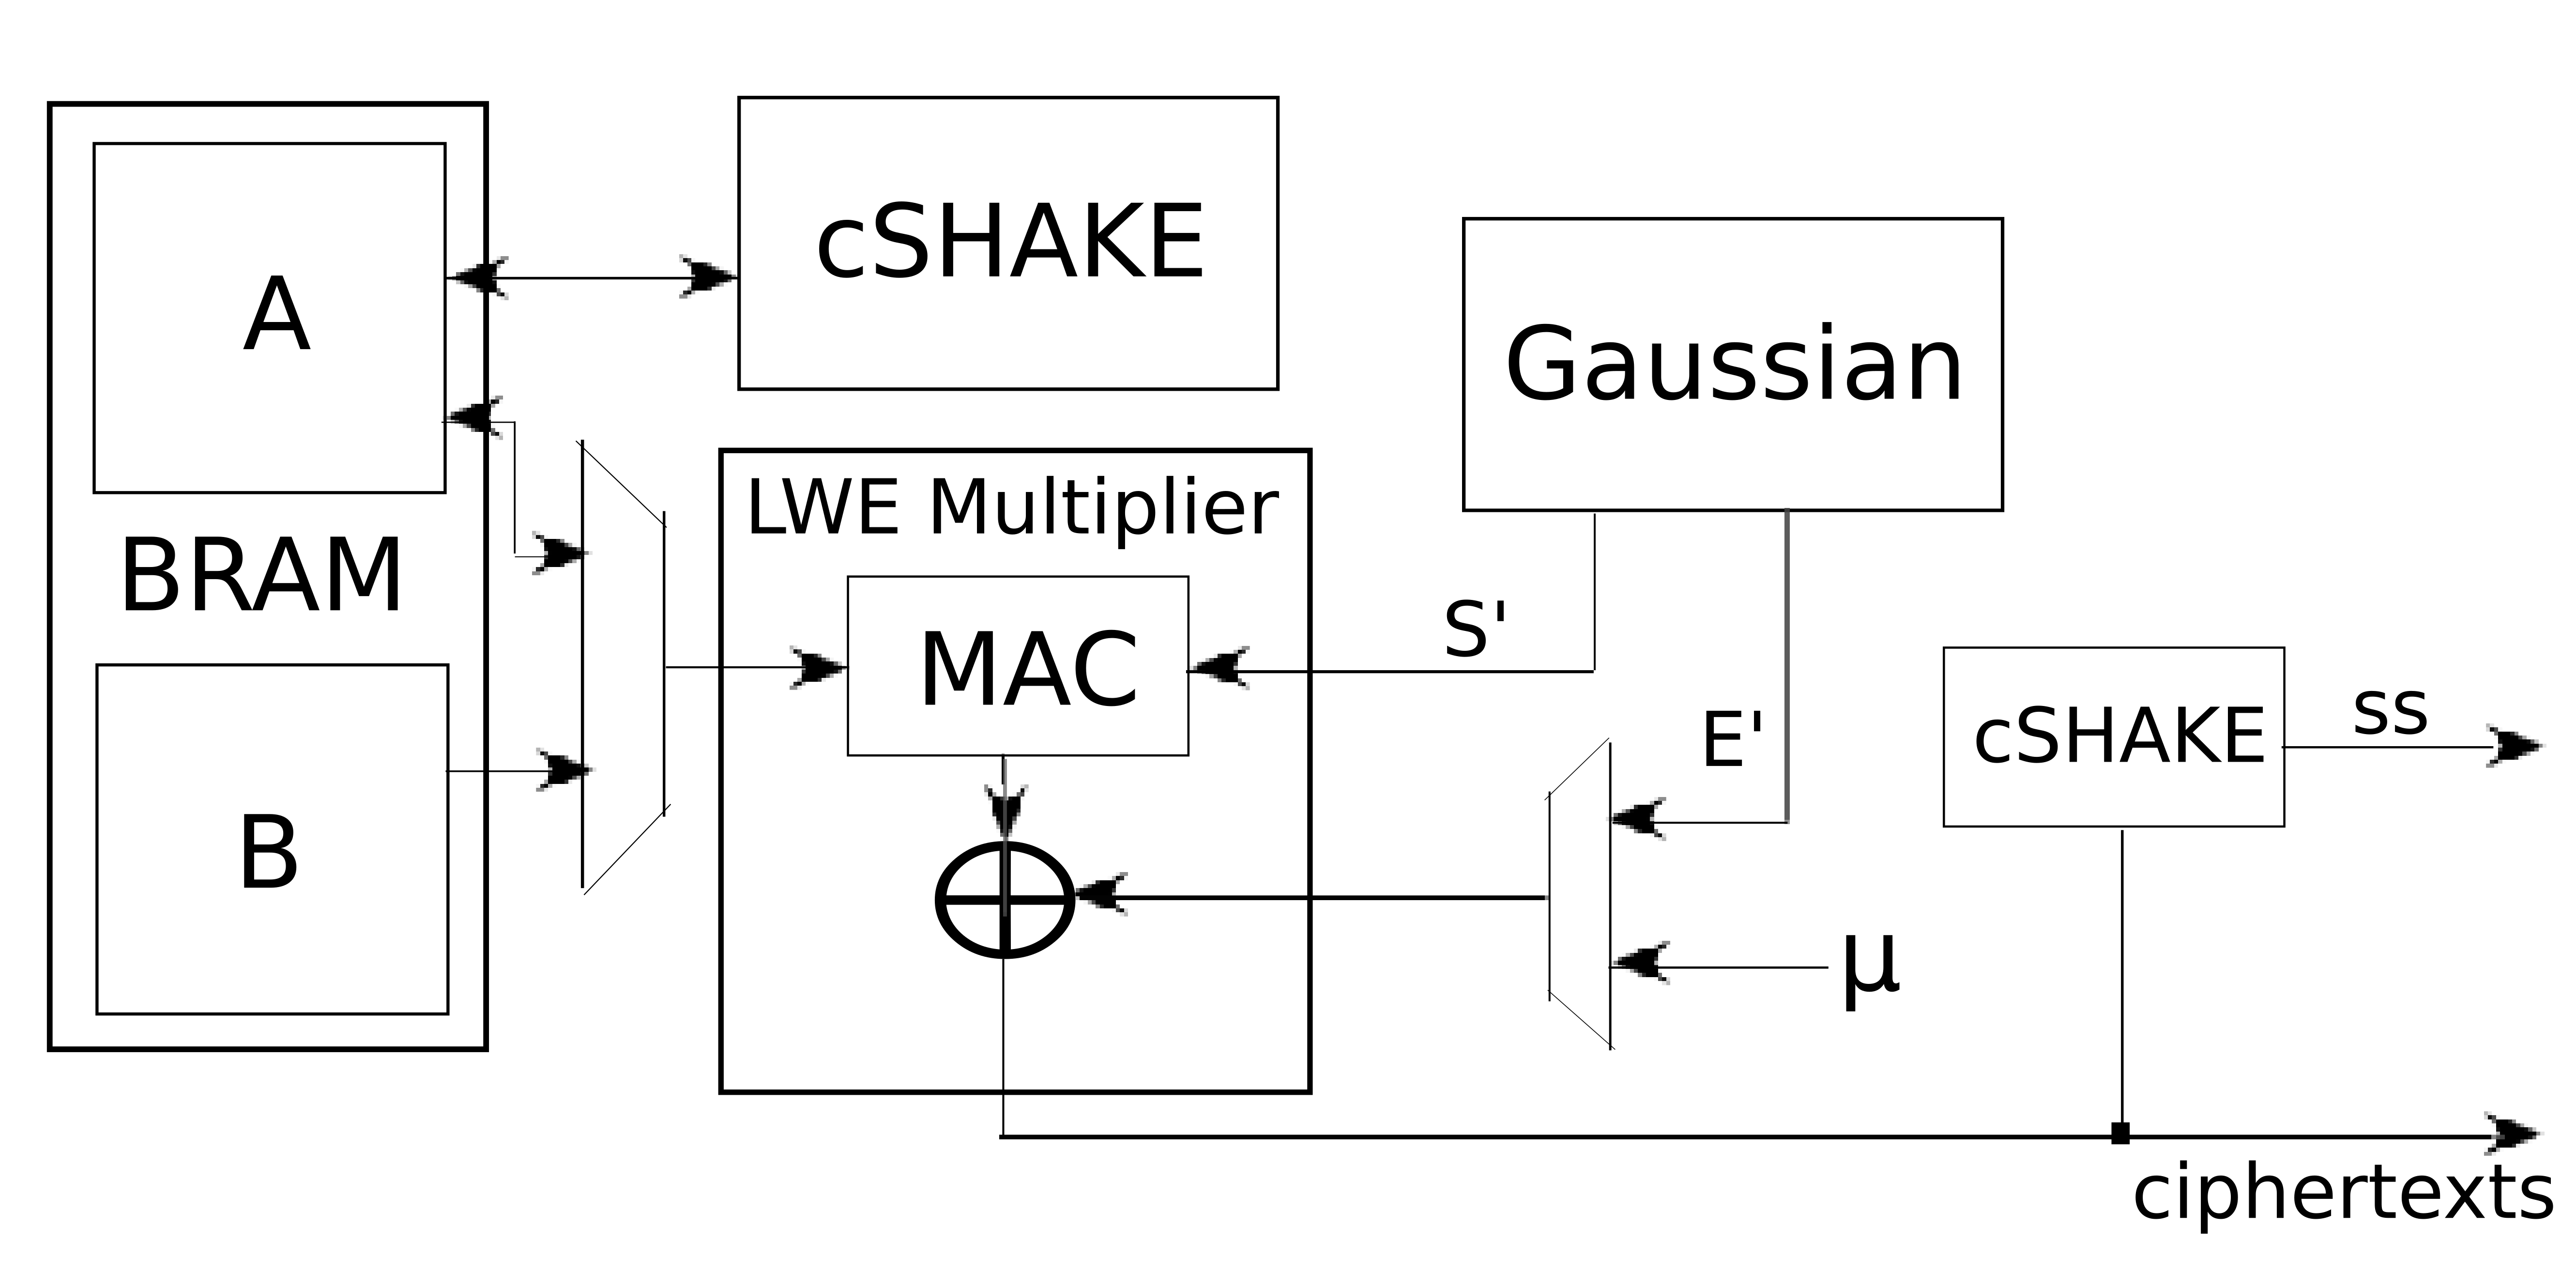
\includegraphics[width=0.95\textwidth,]{figures/FPGA_encaps.png}
  	\caption{A high-level architecture of the FPGA design of \textsf{FrodoKEM-cSHAKE} Encaps.}
  	\label{fig:fpga}
  \end{figure}

\subsection{Additional Modules}

The generation of the deterministic matrix $\mathbf{A}$ uses cSHAKE. For the cSHAKE implementation, a balanced design is used which is based around the mid-range core of KECCAK\footnote{See \url{https://keccak.team/2012/mid_range_hw.html} for more information on the core.}. Due to the deterministic nature of the matrix $\mathbf{A}$, it does not need to be stored in its entirety. This is essential, as otherwise the storage requirements would exceed the capacity of the FPGA, even for the smaller parameter set. Instead, enough of the matrix is pre-generated during the initialization stage, where the remaining matrix is generated on-the-fly, which continuously reuses the same memory blocks. This is similar to the page-flip technique used for $\mathbf{S}^\prime$. This module runs in parallel to the LWE multiplication core and is thus not apart of the critical path and the clock cycle counts of the operations. 

Error sampling is another important module within \textsf{FrodoKEM}. Both \textsf{FrodoKEM-640} and \textsf{FrodoKEM-976} parameter sets require a slightly different distribution, however the standard deviations are close enough to essentially utilize the same FPGA area and performance. A large number of samples are required during a run of \textsf{FrodoKEM}, due to this a fast but rather large sampler is designed in order to keep up with the LWE multiplier. Instead of using a binary search for the table look-up, a large number of comparators are used in order to instantly output an error distribution value in the look-up table.

%This architecture is somewhat shared for Decaps which requires more BRAM storage.

%Most of the remaining operations in Frodo, such as packing, unpacking, modular reduction, encoding, and decoding, happen for free or in cheap parallel processes. The packing process happens naturally d

%Modular reduction is for free!

%Gaussian sampler uses a fast design...